\paragraph{Цель работы:} Знакомство с симулятором станка с УЧПУ Ирис М64, изучение позиционирования и привязки инструментов.

\subsection*{Выполнение}

\begin{enumerate}
    \item Знакомство с интерфейсом симулятора, задание параметров заготовки (рисунок \ref{fig:zag}).
    \item Установка режущего инструмента в гнезда револьверной головки (рисунок \ref{fig:tools}).
    \item Определение координат нулевой точки детали.
        \subitem Переход в режим ZRN, выбор оси (Х, Z) и перемещение инструмента в крайнее положение.
        \subitem Подведение инструмента к заготовке при помощи режимов JOG и HANDLE по оси Z (рисунок \ref{fig:z}).
        \subitem Ввод координат нулевой точки осуществляется при помощи меню ``Tool Param'' $\to$ ``WORK'' (рисунок \ref{fig:coordinates}).
        \subitem Аналогично осуществляется подведение инструмента к заготовке по оси X, окончательная координата расчитывается по формуле \ref{eq:x} (рисунок \ref{fig:x}):
        \begin{equation}\label{eq:x}
            X_0 = X - (R \cdot 2) = 20 - 280 = -260
        \end{equation}
        \subitem Для проверки осуществляется переход в нулевую точку: переключение в режим MDI и строки кода (рисунок \ref{fig:goto}), используя выражение:
        \begin{verbatim}
        G54 T0101 G00 X0Z0
        \end{verbatim}
    \item Привязка (коррекция) инструмента.
        \subitem Коррекция инструмента осуществляется путем подведения инструмента к заготовке в режиме JOG и вычислением расстояния между нулевой точкой и точкой текущего положения инструмента.
        \subitem Коррекция на длину осуществляется по формуле \ref{eq:length} (рисунок \ref{fig:length}):
        \begin{equation}\label{eq:length}
            Z_K = |Z_0| - |Z_M| = 295,8 - 159,9 = 135,9
        \end{equation}
        \subitem Коррекция на радиус осуществляется по формуле \ref{eq:radius} (рисунок \ref{fig:radius}):
        \begin{equation}\label{eq:radius}
            X_K = X_0 - X_M + 2 \cdot R = -260 - (-462) + 30 = 232
        \end{equation}
\end{enumerate}

Скриншоты выполнения лабораторной работы прилагаются в приложении А.

\subsection*{Выводы}

Программный пакет ``SSCNC'' является симулятором систем ЧПУ с широкими возможностями визуализации технологического процесса. В лабораторной работе мы изучили интерфейс программы, а также изучили режимы настройки УЧПУ EZMotion-NC 60 T и произвели коррекцию начальной точки для различных инструментов.

\clearpage

\subsection*{Приложение А}

\begin{figure}[ht]
\centering
	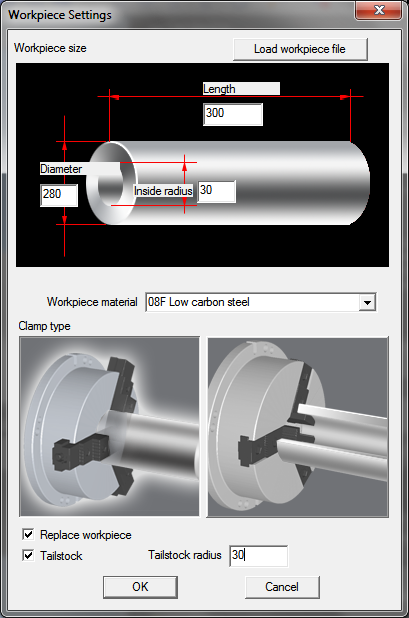
\includegraphics[scale=0.55]{1.png}
    \caption{Задание параметров заготовки\label{fig:zag}}
\end{figure}

\begin{figure}[ht]
\centering
    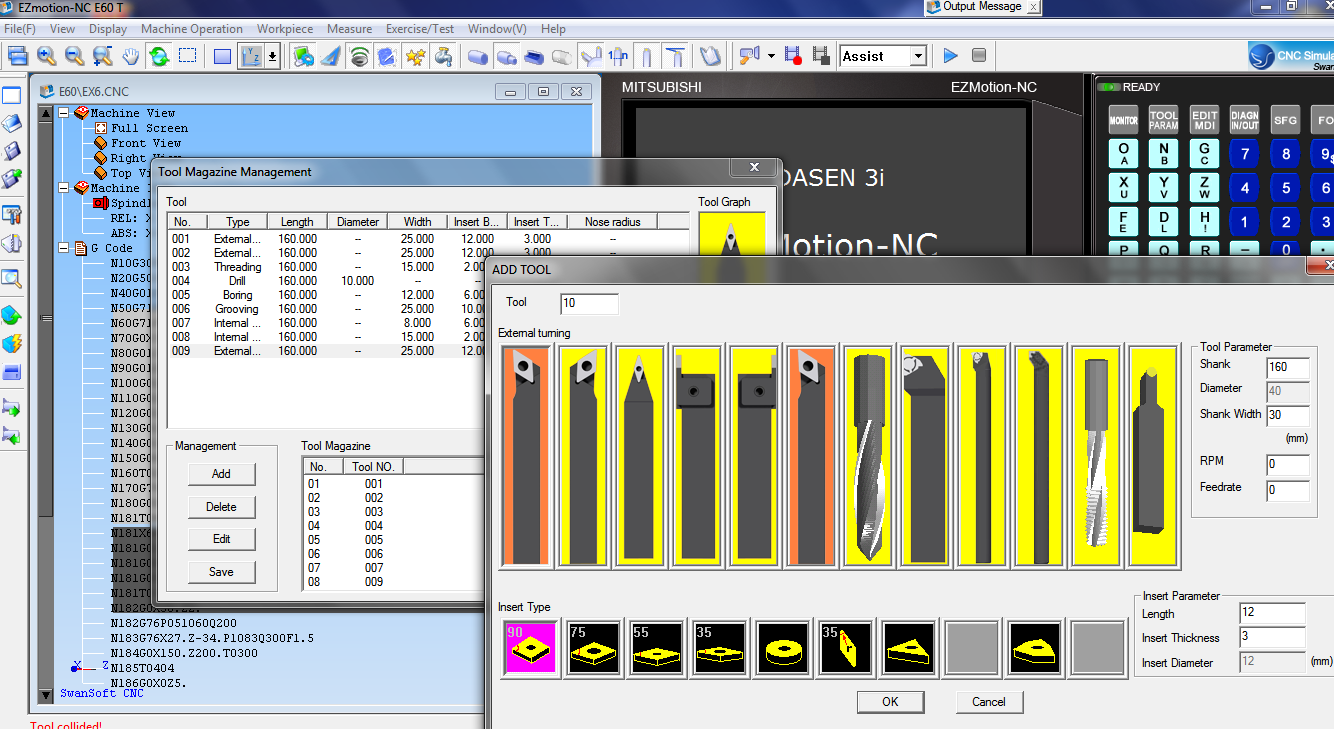
\includegraphics[scale=0.4]{8.png}
    \caption{Установка режущего инструмента в гнезда револьверной головки\label{fig:tools}}
\end{figure}

\begin{figure}[ht]
\centering
	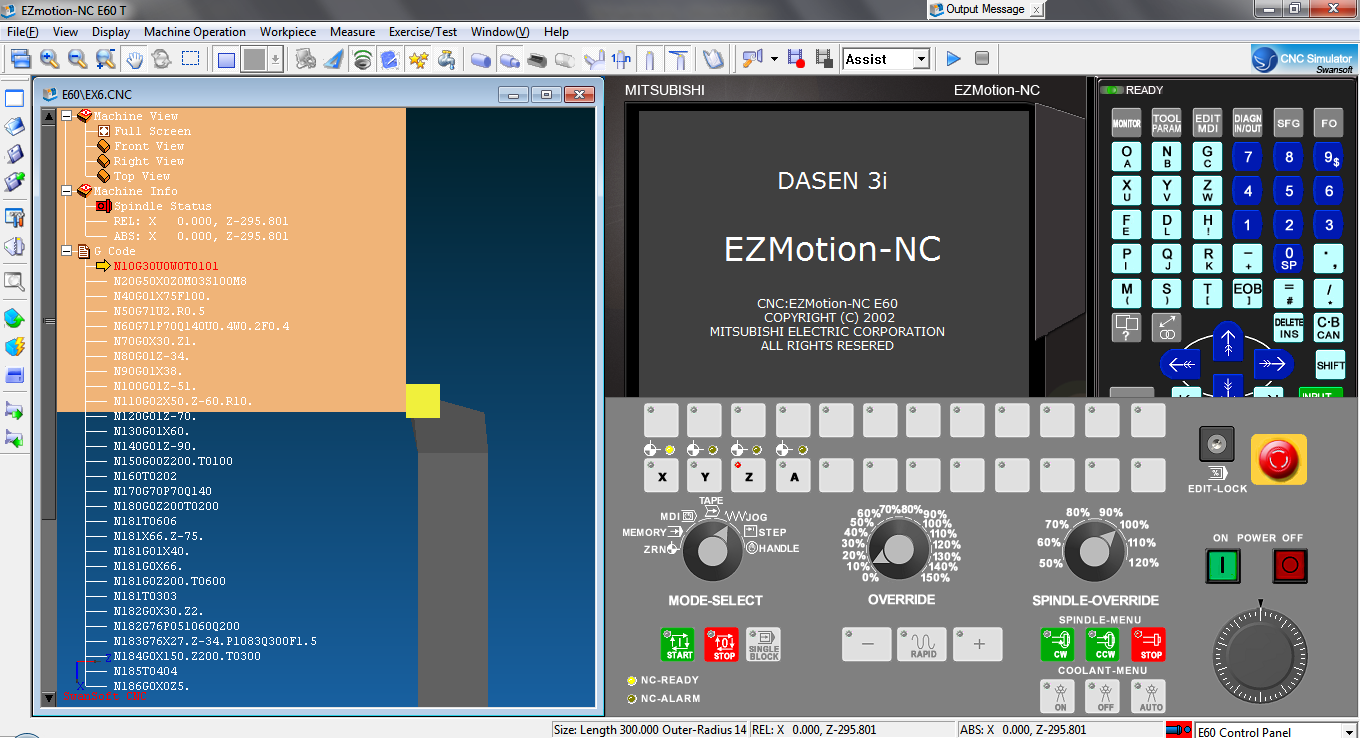
\includegraphics[scale=0.45]{2.png}
    \caption{Подвод инструмента к заготовке по оси Z\label{fig:z}}
\end{figure}

\begin{figure}[ht]
\centering
	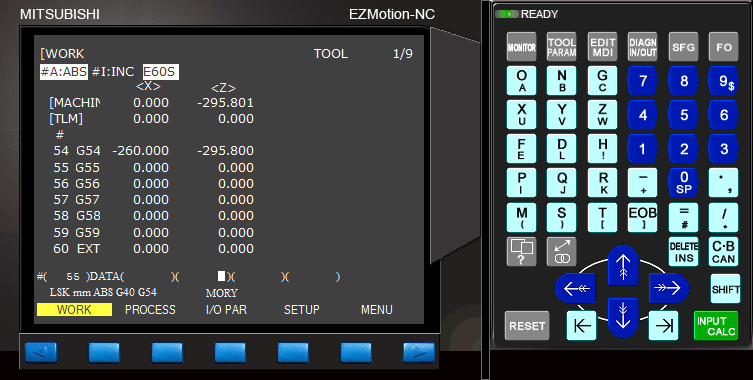
\includegraphics[scale=0.8]{3.png}
    \caption{Координаты нулевой точки\label{fig:coordinates}}
\end{figure}

\begin{figure}[ht]
\centering
	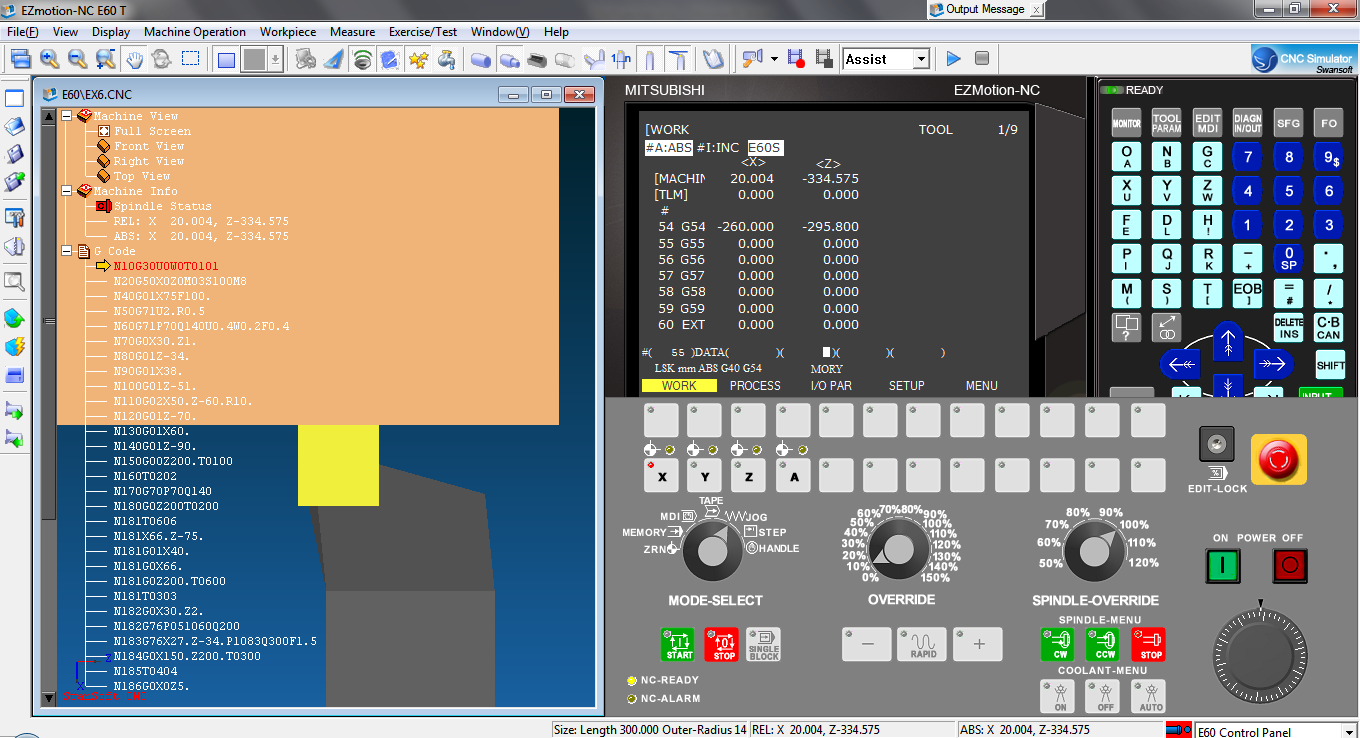
\includegraphics[scale=0.45]{4.png}
    \caption{Подвод инструмента по оси X\label{fig:x}}
\end{figure}

\begin{figure}[ht]
\centering
	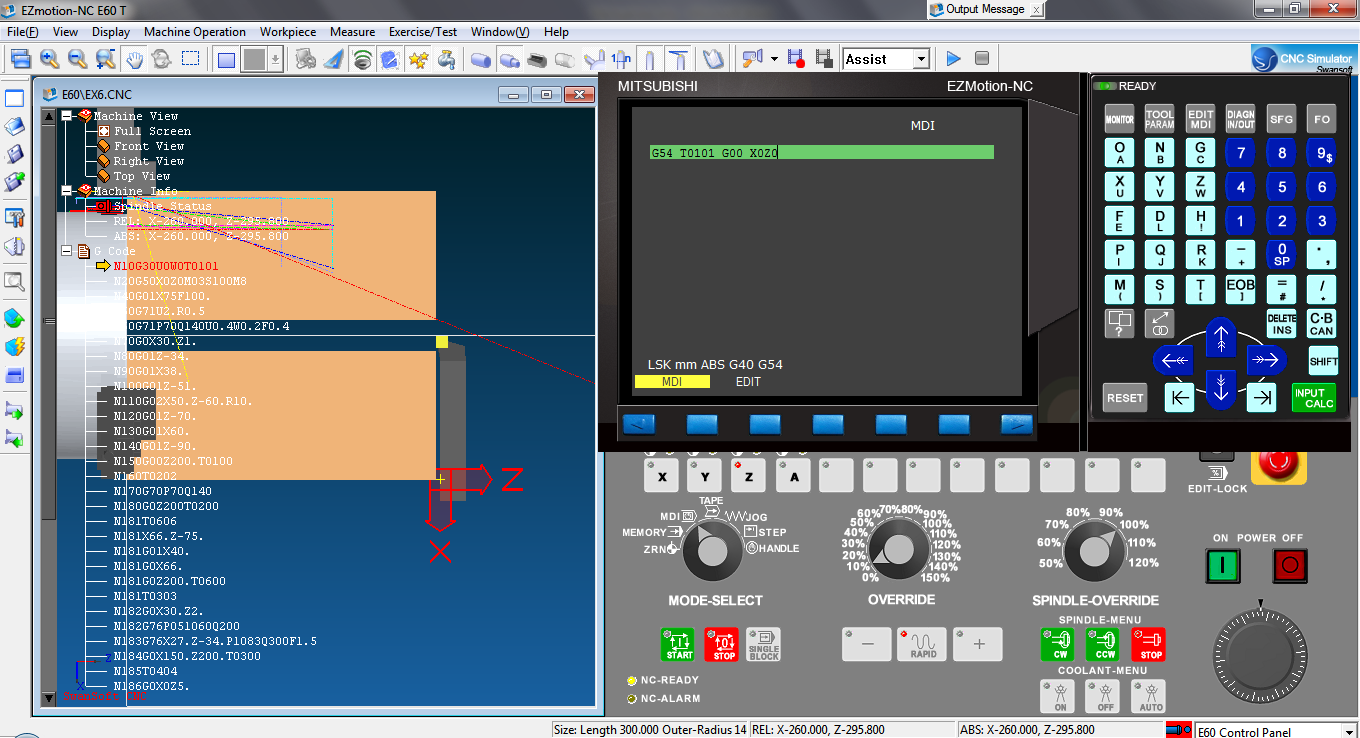
\includegraphics[scale=0.45]{5.png}
    \caption{Переход в нулевую точку\label{fig:goto}}
\end{figure}

\begin{figure}[ht]
\centering
	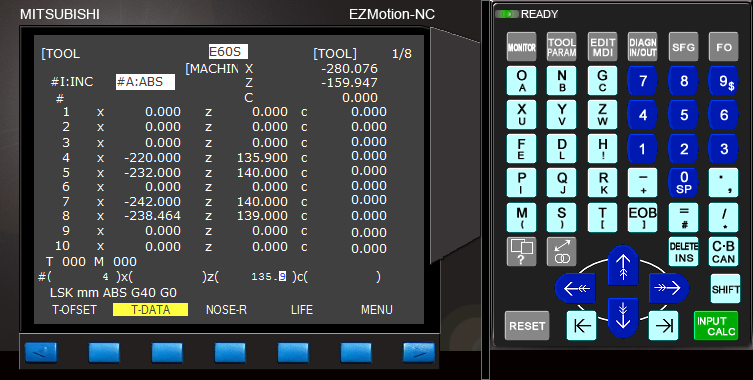
\includegraphics[scale=0.8]{6.png}
    \caption{Коррекция сверла на длину\label{fig:length}}
\end{figure}

\begin{figure}[ht]
\centering
	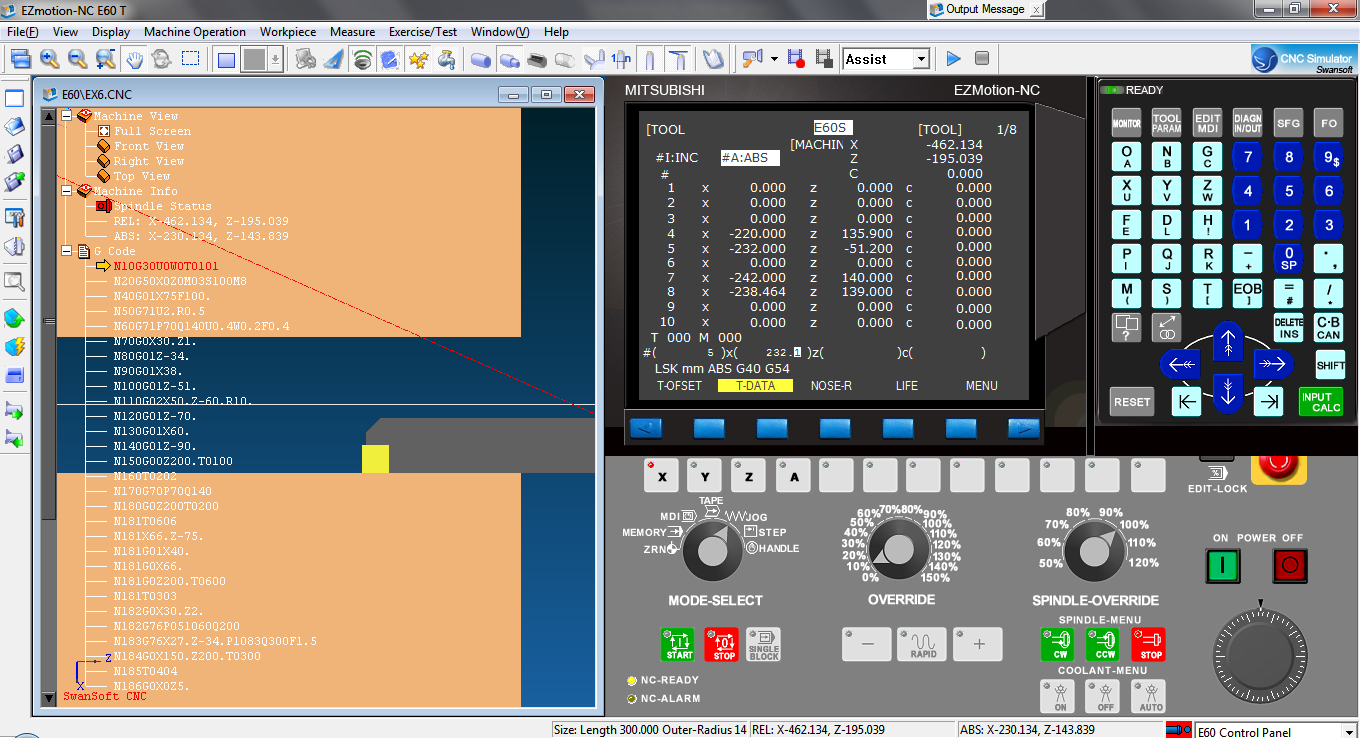
\includegraphics[scale=0.45]{7.png}
    \caption{Коррекция расточного резца на радиус\label{fig:radius}}
\end{figure}
\clearpage
